\section{Methods}
\subsection{Mechanical transfer}
Mechanical transfer relates to the method of moving a sample from one substrate to another whilst minimising the amount of imperfections introduced. This transfer is usually from the growth substrate to a target substrate used for an electrical device or to a TEM grid for characterization in a transmission electron microscope.
\subsection{TEM / EMPAD / EELS? / HRTEM}
\begin{enumerate}
    \item Electron microscope workings and explanation of all detectors
    \item empad detector working / uses
    \item CoM for electric and magnetic fields
    \item charge density mapping
    \item Strain mapping
\end{enumerate}

\subsection{The Transmission electron microscope}
The Transmission electron microscope (TEM) is a microscope that far exceeds the capabilities of a normal light microscope. Both types of microscope use a series of lenses to magnify the image of a specimen.
A normal light microscope can amplify an image up to about 1500$\times$ and is limited by the diffraction limit of light. Assuming an average wavelength of \SI{550}{\nm} for green light, a high-end microscope is limited to resolving features \SI{100}{\nm} apart.
This limit is insufficient for looking at atomic structures \cite{PhysRevLett.106.193905}.\\
An electron microscope circumvents this limit by using electrons, not light, to probe the specimen. Electrons when accelerated have a smaller wavelength than light thus allowing for images with resolved features as small as \SI{0.05}{\nm}. \cite{kisielowski_freitag_bischoff_van}
The TEM works by releasing electrons from an electron source and accelerating them to an energy typically expressed in kilo-electronvolt; as shown in equation \ref{eq:acc_volts}, the higher the accelerating voltage of the microscope the smaller the de Broglie wavelength of an electron, which results in a higher resolving power. Modern electron microscopes accelerate electrons up to \SI{300}{\kilo \electronvolt}

\begin{equation}
    \lambda_e = h\cdot \left[ 2 \cdot e \cdot m_e \cdot V_a \right]^{-1/2}
    \label{eq:acc_volts}
\end{equation}

\begin{figure}[h]
    \centering
    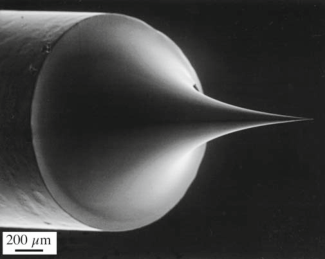
\includegraphics[keepaspectratio, width=0.5\linewidth]{resources/Figures/feg.png} 
    \caption{Pictured is the tip of a field emission gun \cite{Williams2009-ww}. The tapered tip facilitates the creation of a strongly varying potential that eases the expulsion of electrons from the material. These electrons are then accelerated along the optical axis.}
    \label{fig:feg}
\end{figure}

In a TEM the electrons are released from a field emission gun (FEG, pictured in Figure \ref{fig:feg}). 
The FEG is placed in proximity to two anodes, the first anode is positively charged to several kilovolts such that it extracts electrons from the tip of the FEG, the second anode is charged to the wanted acceleration voltage \cite{Williams2009-ww}.
FEGs are about three orders of magnitude brighter than thermionic emission electron sources \cite{field-emission}.
After being emitted the electrons pass through a monochromator that reduces the energy spread of the emitted electrons. An electron then continues along the optical axis into an illuminating system consisting of multiple electromagnetic lenses, which lenses are activated and to what extent depends on the operating mode of the electron microscope.

\subsubsection{Bright Field}
A bright field (BF) image of the sample is acquired by using a parallel electron beam. This beam is formed using the lens configuration shown in figure \ref{fig:tem_operating}. This parallel beam is typically several micrometers in size at magnifications up to 20k-100k$\times$.
In normal operating mode a BF image is captured by a camera looking at a phosphorous screen or by a camera directly, this method of imaging is most analogues to a normal light microscope.
The electron beam is focused in such a way that it illuminates the sample with a parallel beam, such a beam is also used for creating the clearest diffraction patterns.
%A bright field image can also be formed in STEM operating mode.
\begin{figure}[h]
    \centering
    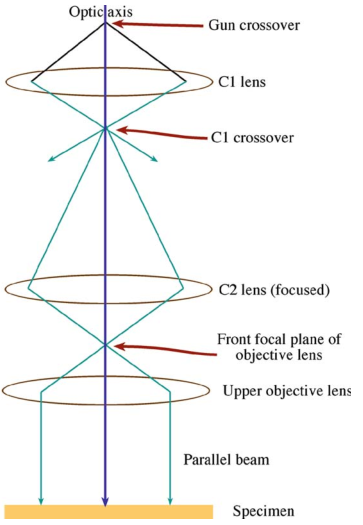
\includegraphics[width=0.3\textwidth, keepaspectratio]{resources/Figures/tem_operating.png}
    \caption{Illumination system for parallel beam.}
    \label{fig:tem_operating}
\end{figure}
\subsubsection{Dark Field, Z-contrast}
For dark field and Z-contrast the electron beam is focused to a small area, this creates a higher intensity electron beam with a probe-like point as can be seen in Figure \ref{fig:stem_operating}. Since all the electrons are focused on a small area there is no contrast information that can be used to form an image. To form an image using such a beam the probe point needs to be scanned over the sample leading to the term Scanning Transmission Electron Microscopy.
Dark field images use electrons scattered away from the optical axis to form an image, to achieve this most STEMs have a series of annular dark field detectors.
These ring shaped detectors encircle the central bright field detector and can collect electrons that have been scattered at various angles. Normal dark field detectors collect electrons scattered up to an angle of \SI{50}{\milli \radian}. The outermost detector is the high-angle annular dark field detector (HAADF) which collects electrons scattered beyond \SI{50}{\milli \radian} and can be used to create Z-contrast (atomic number Z) or mass-thickness images.
The HAADF detector is used since the electrons it collects are almost exclusively incoherently elastically scattered which is proportional to the atomic number Z.
The scanning beam then gathers this atomic number information as intensity information for every probe position in the sample.
Layering two monolayers such that the atoms are aligned, and the probe is perpendicularly incident on the sample will sum the intensity of the two atomic weights of the stacked atoms in the image. The stacking pattern can then be determined by looking at a line plot of the atomic mass over atoms.  
\begin{figure}[h]
    \centering
    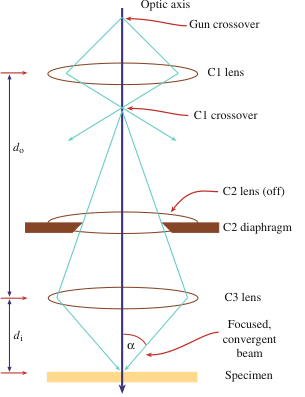
\includegraphics[width=0.5\textwidth, keepaspectratio]{resources/Figures/stem_operating.png}
    \caption{Illumination system for convergent beam.}
    \label{fig:stem_operating}
\end{figure}

\subsubsection{Energy-dispersive x-ray spectroscopy}
Pagina 581 W\&C

\begin{figure}
    \def\svgwidth{.66\linewidth}
    \import{resources/Figures}{Titan_full_column.pdf_tex}
    
\end{figure}

\subsubsection{Electron microscope pixel-array detector}
%In TEM operating mode a parallel electron beam is used to illuminate the sample and form an image on either the phosphorous screen or digital camera, this spreads the beam over a larger area such that the local electron dose is relatively uniform.
In a scanning-TEM (STEM) mode the beam is focused to a small probe-like point at the specimen. Elastic scattering then deflects the electrons from the optical axis onto one of the ring shaped detectors encircling the optical axis, these detectors are called the dark field detectors. These singular annular detectors bunch the elastically scattered electrons together, losing valuable information on the exact scattering angle. The electron microscope pixel-array detector (EMPAD) solves this problem by replacing the annular dark field and singular bright field detectors with a single fast-readout, high dynamic range pixel grid on which every pixels' electron dose is stored separately such that after acquisition of a complete STEM scan the bright- and dark-field detectors can be virtually recreated by integrating the electron dose using annular or circular masks on the data. A greater accuracy in scattering angle is also available since every pixel in the array has its own smaller range of scattering angles whose electrons the pixel collects.



\subsubsection{Electron energy-loss spectroscopy}
In a TEM setup electrons are essentially shot through a sample in which the electrons can either simply pass through or scatter, in the latter scenario there are two possibilities, electrons can scatter elastically or inelastically.
Scattering is a result of the interaction between the sampling electrons from the TEM source and the charged particles in the specimen.\\
When scattering elastically the electrons interact with a nucleus of the specimen whose mass is many times greater than that of the sampling electron, resulting in a small and usually unmeasurable energy transfer.
In a crystalline specimen electrons can only be scattered at certain angles due to the crystal structure creating a diffraction pattern of bright spots. In cases of large scattering angles the electron does transfer a significant amount of energy and can even reverse direction, this energy transfer can permanently displace atoms in the crystal structure causing a defect.\cite{Egerton_2008}\\
When the sampling electron interacts with an electron in the specimen's crystal lattice inelastic occurs due tot the similarity in mass between the two electrons. The energy transfer of this interaction ranges from a few electronvolts up to multiple hundreds of electronvolts.
Inelastic scattering not only results in an energy transfer but also in a momentum transfer as shown in figure \ref{fig:scat}, the $k'$-vector shows a scattered electron that deviates from the not scattered electron vector $k_0$.
The total momentum transfer is the sum of the perpendicular momentum transfer $q_{\perp}$ proportional to the scattering angle $\theta$ and the momentum transfer parallel to the undisturbed path due to an energy transfer from the sampling electron to the sample. This parallel momentum transfer is thus proportional to the energy loss of the electron.
Figure \ref{fig:bands} shows the band structure of the crystalline sample of which the electrons scatter. In this figure two dispersion bands are shown, both bands can be occupied by electrons of certain energies, to excite an electron from the blue band to the red band an electron needs either energy (path $t_1$) or energy and momentum (path $t_2$).
The needed energy and momentum are transferred from an incident sampling electron in the inelastic interaction. By measuring the energy and momentum of a scattered electron it is possible to piece together all the combinations of energy and momenta transfer possible and thus find the band structure of the sample.\\
Another form of inelastic scattering is plasmon excitation.\\
Since the outer-shell electrons of an atom are only weakly bound to the nucleus due to screening effects but are coupled together by electrostatic interaction. These delocalised electrons form an energy band similar to that shown in figure \ref{fig:bands}.
When a fast-moving sampling electron is shot through the sample all nearby outer-shell electrons are displaced. If the sampling electron's velocity exceeds the fermi speed the displacement of outer-shell electrons creates an oscillating ripple creating waves of alternating positive and negative electric charge, this is known as a plasmon wake.\cite{Egerton_2008}

\subsection{Momentum resolved electron energy-loss spectroscopy}
\label{sec:MREELS}
Momentum resolved electron energy-loss spectroscopy hereafter abbreviated as MREELS is a TEM imaging technique in which the imaging plane of the CCD camera is placed in the focal point of the imaging lenses and energy filter.
This allows the camera to take a diffraction mode image in which the diffraction pattern of the scattering electrons is shown. This is illustrated in figure \ref{fig:diff-im}. In this figure the crystalline sample is shown as the box with the slanted lines that represent the Miller planes of the crystal structure.
As shown in the figure all electrons that scatter of the same family of Miller planes get focused on the same region on the imaging sensor, electrons that do not scatter also get focused in one spot at the centre of the diffraction pattern.
A diffraction mode image does not image normal space but instead shows reciprocal space which is also the reason this type of image is useful. In a normal image one would attribute lengths to the axes of an image but in a diffraction mode image the separation of features is given by a momentum difference.
The separation of the light and dark grey arrows on the imaging plane in figure \ref{fig:diff-im} is thus equal to the difference in perpendicular momentum transfer between scattering electrons (light grey) and electrons that do not scatter (dark grey), a 3D representation is presented in the Appendix.
Since the momentum transfer for the electrons that do not scatter is zero the momentum transfer for scattering of a certain family of planes can be determined.

\subsubsection{Energy filtered transmission electron microscope}
\label{sec:eftem}
An energy filtered transmission electron microscope is a microscope with an energy filter placed in the optical column of the TEM. Energy filtering is accomplished by the use of electromagnetic prisms such as those shown in figure \ref{fig:filter}.
These prisms just like ordinary prism disperse the electrons with different wavelengths which are proportional to electron energy. By sliding a slit into the cone of dispersed electrons it is possible to choose a finite range of electron energies to image.
The EFTEM setup can be used in conjunction with the MREELS imaging technique to gather information on both the momentum transfer of the electron (via MREELS) and the energy loss associated (via EFTEM) with that momentum transfer.






\subsection{Data analysis}
\subsubsection{CoM analysis}
\subsubsection{Charge density analysis}
\subsubsection{Strain analysis}




